\documentclass[Bachelorarbeit.tex]{subfiles}
\begin{document}

\graphicspath{{./figures/newMarket/}}	%specifying the folder for the figures

\chapter{A new Market}
\label{ch:newMarket}
As already introduced in section \ref{ch:interpretation_reenablingTrading} a new market is necessary to repair the miss-allocation of collateralized assets in the range of the pessimist agents by enabling the agents to trade collateralized assets against cash.

\section{Definition}
\subsection{Products}
Collateralized assets are traded against cash. The buyer gets a specific amount of collateralized assets for a given amount of cash where the seller gives away the specific amount of collateralized assets and gets the given amount of cash.

\subsection{Price-Range}
As within all other three markets the price-ranges of the offers must be defined. Note that all prices must be obviously in the unit of cash according to the previously defined products.

\paragraph{minimum}
When calculating the minimum price of a collateralized asset - that is how much is the collateralized asset minimally worth - it is important to include the collateral-aspect of the asset. Thus one starts with the minimum asset-price in cash which is the down-price \textit{pD} and subtracts the minimum amount of cash which is bound through a bond as collateral which is \textit{pD}. This value is a constant for all agents.

\begin{equation}
\textit{min collateralized asset-price} = \textit{pD} - \textit{pD} = 0
\end{equation}
 
\paragraph{maximum}
To calculate the maximum price of a collateralized asset - that is how much is the collateralized asset maximally worth - one needs to include the collateral-aspect of the asset too. Equal to calculating the minimum one starts now with the maximum asset-price in cash which is the up-price \textit{pU} and subtracts the maximum possible amount of cash which is bound through a bond as collateral which is the face-value \textit{V}. This value is a constant for all agents.

\begin{equation}
\textit{max collateralized asset-price} = \textit{pU} - \textit{V}
\end{equation}

\paragraph{limit}
Applying the same rules as in minimum and maximum to the limit price calculation one needs to subract the limit-price of loans from the limit-price of asset to receive the limit-price of a collateralized asset. This value is individual for each agent as the limit-prices differ across the agents both for assets and loans.

\begin{equation}
\textit{limit-price of collateralized asset} = \textit{limit-price of asset} - \textit{limit-price of loan}
\end{equation}

\subsection{Bid-Offering}
The way bid-offers are generated is very similar to the Bond/Cash market. Bid offers are generated only when the agent has any cash holdings. The price is drawn randomly between the minimum price and the limit-price because when buying one wants to buy below the expected value to make a profit. As amount one TRADING-UNIT of an asset is selected - in the thesis-implementation 0.1 - but if there is not enough cash left to buy one TRADING-UNIT of assets then the amount of assets is selected which can be bought with the remaining cash holdings.

\begin{table}[H]
	\centering
	\caption{Bid-Offering parameters}
	\begin{tabular} { l c r }
		\hline
		Pre-Condition & $\textit{cash holdings} > 0$  \\
		Asset-Price & $\mathrm{random}(\textit{min coll. asset-price}, \textit{limit-price of coll. asset})$ \\
		Asset-Amount & $\min ( \frac{ \textit{cash holdings} }{ \textit{Asset-Price} }, \textit{TRADING-UNIT} )$ \\
		\hline
	\end{tabular}
\end{table}


\subsection{Ask-Offering}
The way ask-offers are generated is very similar to the Bond/Cash market. Ask offers are generated only when the agent has any collateralized assets. The price is drawn randomly between the limit-price and maximum price because when selling one wants to sell above the expected value to make a profit. As amount one TRADING-UNIT of an asset is selected - in the thesis-implementation 0.1 - but if there are fewer collateralized assets left then the remaining amount of collateral is selected.
See Chapter \ref{ch:implementation} for the equation of collateral holdings.

\begin{table}[H]
	\centering
	\caption{Ask-Offering parameters}
	\begin{tabular} { l c r }
		\hline
		Pre-Condition & $\textit{collateralized assets} > 0$  \\
		Asset-Price & $\mathrm{random}(\textit{limit-price of coll. asset}, \textit{max coll. asset-price})$ \\
		Asset-Amount & $\min ( { \textit{collateralized assets} }, \textit{TRADING-UNIT} )$ \\
		\hline
	\end{tabular}
\end{table}

\subsection{Match}
Below the wealth-exchange table is given in case of a match between two agents on the new market. Note that the wealth is increased/decreased as given by the +/- signs.

\begin{table}[H]
	\centering
	\caption{Wealth-Exchange on match}
	\begin{tabular} { l c c }
		& Seller & Buyer \\
		\hline
		Loan Given & + matching-amount & N/A \\
		Loans Taken & N/A & - matching-amount \\
		Assets holdings & - matching-amount & + matching-amount \\
		Cash holdings  & + matching-price & - matching-price \\
		\hline
	\end{tabular}
\end{table}

\section{Results}
Of most importance are the results of the simulation when using the new market. The plain results are given in this section where the interpretation of the results are given in the following section.

\medskip

As experiment-configuration the same is used as given in Chapter \ref{ch:results} except that the new market is now activated too.

\begin{table}[H]
	\centering
	\caption{Configuration for all experiments}
	\begin{tabular} { l c r }
		\hline
		Agent-Count & 100 \\
		Bond-Type & 0.5 \\
		Replication-Count & 50 \\
		Matching-Round & max. 500 offering-rounds \\
		Terminate after & 1000 failed successive matching-rounds \\
		\hline
	\end{tabular}
\end{table}

\subsection{Fully-Connected topology}

\begin{figure}[H]
	\centering
  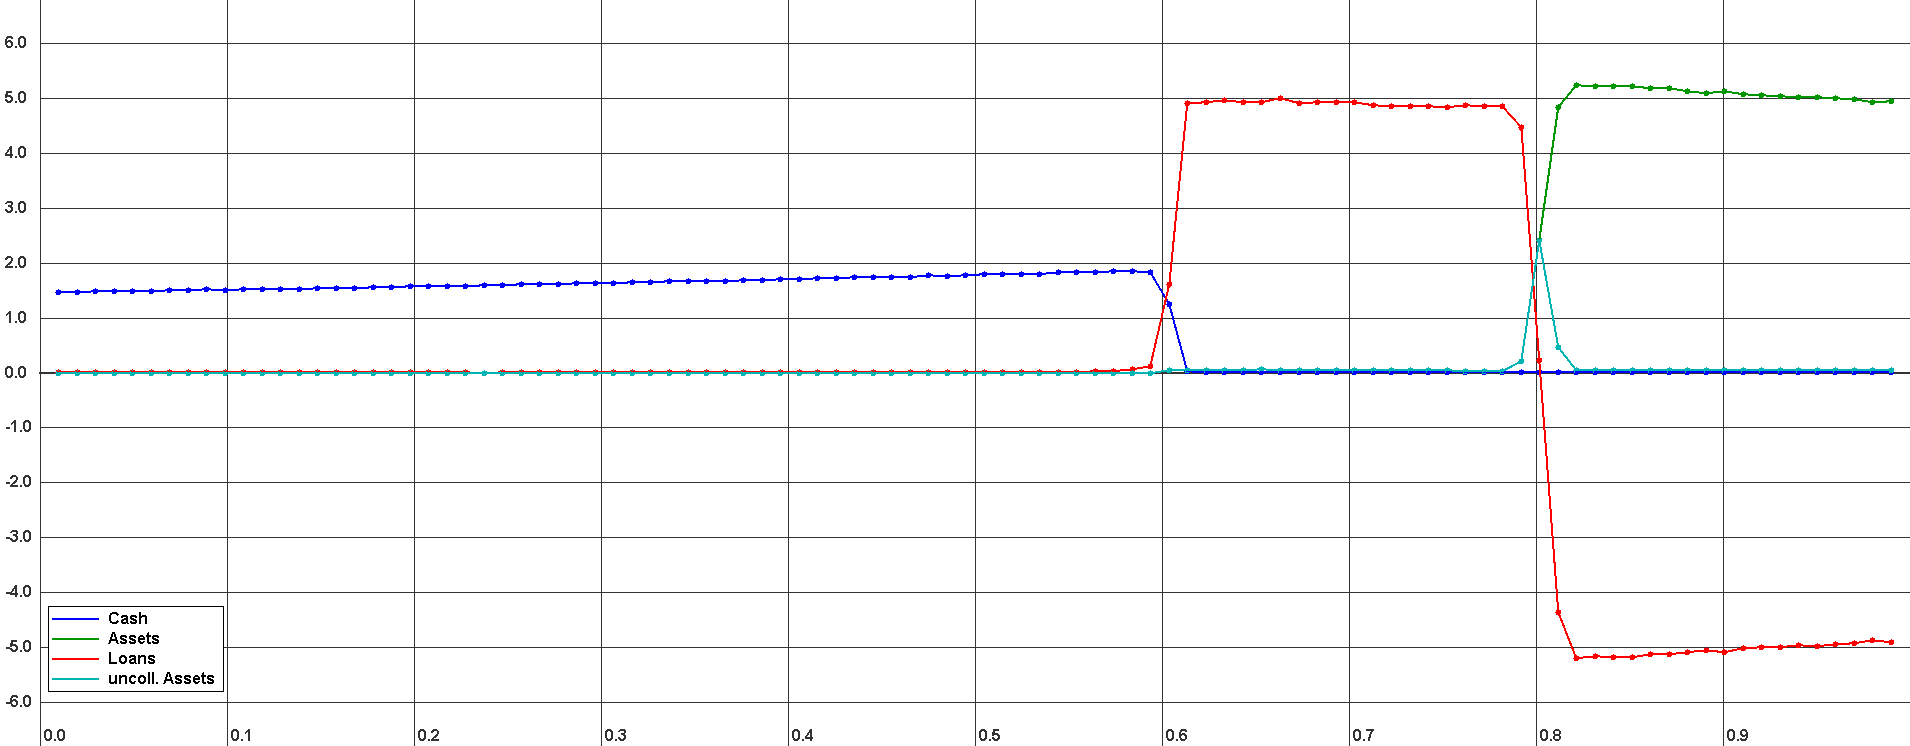
\includegraphics[width=1.0\textwidth, angle=0]{FULLYCONNECTED_100_WITHCOLLATERALMARKET_REPL.png}
	\caption{Wealth-Distribution of Fully-Connected topology with Collateral/Cash market}
	\label{fig:wealth_FULLYCONNECTED_100_WITHCOLLATERALMARKET_REPL}
\end{figure}

\begin{table}[H]
	\caption{Equilibrium of Fully-Connected topology with Collateral/Cash market}
	\centering
	\begin{tabular} { l c r }
		\hline
		Asset-Price p & 0.688 (0.008) \\
		Bond-Price q & 0.381 (0.002) \\
		Marginal Agent i1 & 0.597 (0.005) \\
		Marginal Agent i2 & 0.803 (0.003) \\
		\hline
		Pessimist Wealth & 1.597 (0.009) \\
		Medianist Wealth & 4.76 (0.1) \\
		Optimist Wealth & 4.963 (0.052) \\
		\hline
	\end{tabular}
\end{table} 

\begin{table}[H]
	\caption{Performance of Fully-Connected topology with Collateral/Cash market}
	\centering
	\begin{tabular} { l c r }
		\hline
		Successful matching-rounds & 1916.14 (31.42) \\
		Failed matching-rounds & 4448.66 (1668.93) \\
		Total matching-rounds & 6364.8 (1679.21) \\
		\hline
		Ratio successful/total & 0.3 \\
		Ratio failed/total & 0.7 \\
		\hline
	\end{tabular}
\end{table}

\begin{table}[H]
	\caption{Difference of Fully-Connected topology to theoretical equilibrium as given in Table \ref{tab:theoretical_equilibrium_100Agents_05Bond} of chapter \ref{ch:results}}
	\centering
	\begin{tabular} { l c c c r }
		& Result & Reference & difference to Reference \\
		\hline
		Asset-Price p & 0.688 & 0.717 & -4.0\% \\
		Bond-Price q & 0.381 & 0.375 & +1.6\% \\
		Marginal Agent i1 & 0.597 & 0.584 & +2.2\% \\
		Marginal Agent i2 & 0.802 & 0.803 & +0.1\% \\
		\hline
	\end{tabular}
\end{table} 

\begin{table}[H]
	\caption{Difference of Fully-Connected topology to equilibrium without Collateral/Cash market as given in Table \ref{tab:fullyconnected_equilibrium_100Agents_05Bond} of chapter \ref{ch:results}}
	\centering
	\begin{tabular} { l c c c r }
		& Result & Reference & difference to Reference \\
		\hline
		Asset-Price p & 0.688 (0.008) & 0.689 (0.01) & -0.1\% (-20\%) \\
		Bond-Price q & 0.381 (0.002) & 0.384 (0.004) & -0.7\% (-50\%) \\
		Marginal Agent i1 & 0.597 (0.005) & 0.603 (0.007) & -1.0\% (-28\%) \\
		Marginal Agent i2 & 0.803 (0.003) & 0.803 (0.003) & 0.0\% (0\%) \\
		\hline
		Pessimist Wealth & 1.597 (0.009) & 1.597 (0.015) & 0.0\% (-40\%) \\
		Medianist Wealth & 4.76 (0.1) & 4.565 (0.113) & +4.2\% (-11\%) \\
		Optimist Wealth & 4.963 (0.052) & 5.021 (0.064) & -1.1\% (-19\%) \\
		\hline
	\end{tabular}
\end{table} 

\subsection{Ascending-Connected topology}
\begin{figure}[H]
	\centering
  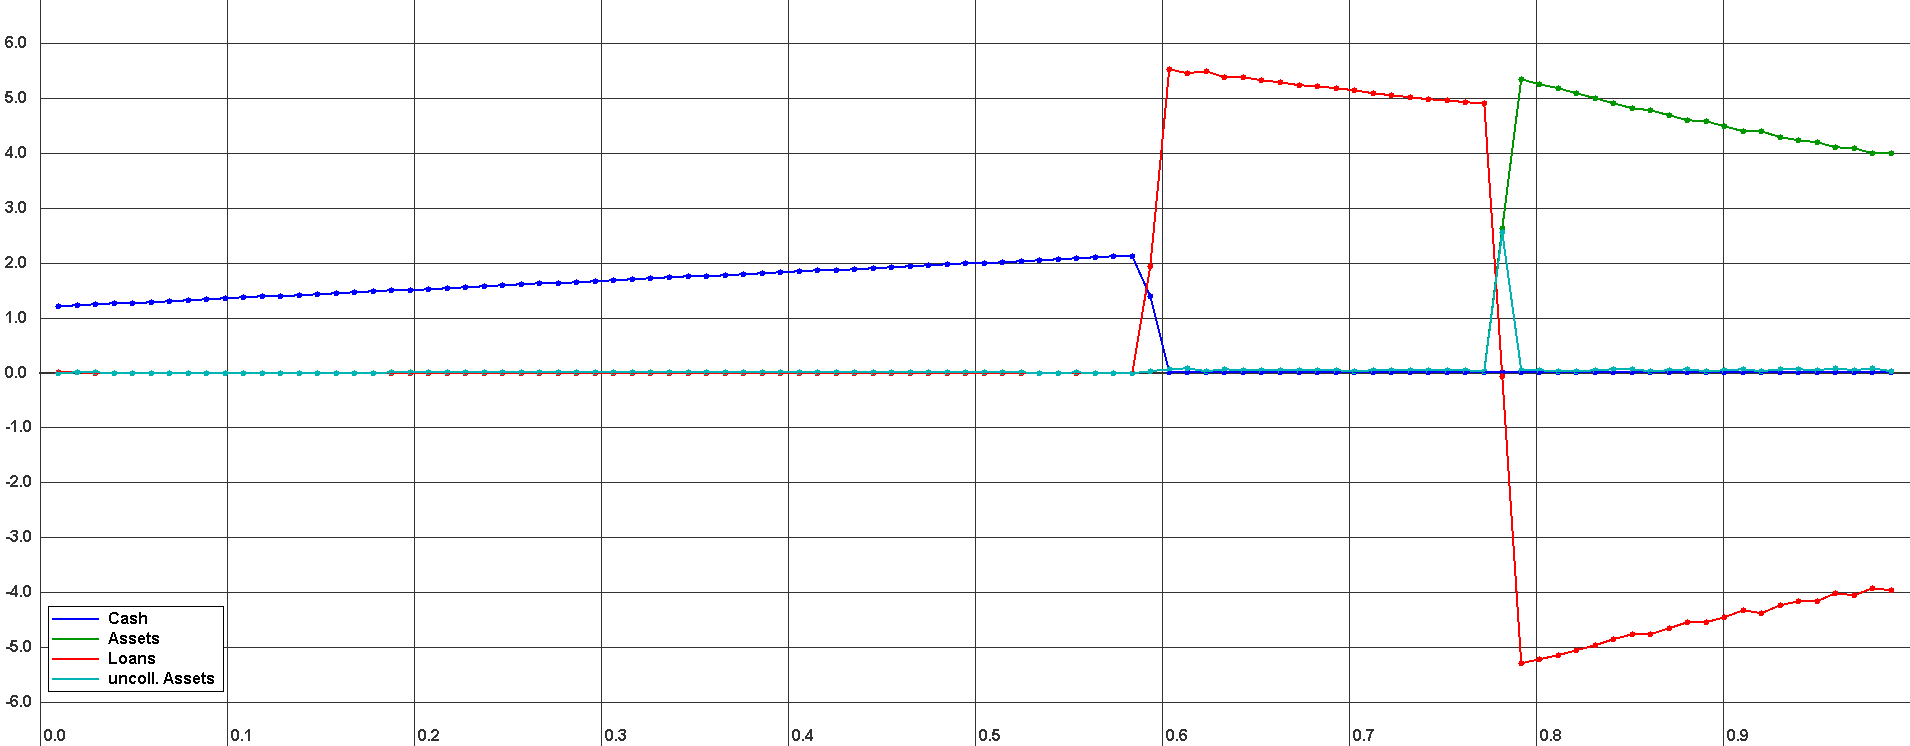
\includegraphics[width=1.0\textwidth, angle=0]{ASCENDINGCONNECTED_100_WITHCOLLATERALMARKET_REPL.png}
	\caption{Wealth-Distribution of Ascending-Connected topology with Collateral/Cash market}
	\label{fig:wealth_ASCENDINGCONNECTED_100_WITHCOLLATERALMARKET_REPL}
\end{figure}

\begin{table}[H]
	\caption{Equilibrium of Ascending-Connected topology}
	\centering
	\begin{tabular} { l c r }
		\hline
		Asset-Price p & 0.713 (0.013) \\
		Bond-Price q & 0.383 (0.005) \\
		Marginal Agent i1 & 0.584 (0.0) \\
		Marginal Agent i2 & 0.782 (0.0) \\
		\hline
		Pessimist Wealth & 1.671 (0.0) \\
		Medianist Wealth & 5.032 (0.013) \\
		Optimist Wealth & 4.508 (0.006) \\
		\hline
	\end{tabular}
\end{table} 

\begin{table}[H]
	\caption{Performance of Ascending-Connected topology}
	\centering
	\begin{tabular} { l c r }
		\hline
		Successful matching-rounds & 51,838.74 (1613.36) \\
		Failed matching-rounds & 1124.76 (28.31) \\
		Total matching-rounds & 52,963.5 (1612.31) \\
		\hline
		Ratio successful/total & 0.98 \\
		Ratio failed/total & 0.02 \\
		\hline
	\end{tabular}
\end{table}

\begin{table}[H]
	\caption{Difference of Ascending-Connected topology to theoretical equilibrium as given in Table \ref{tab:theoretical_equilibrium_100Agents_05Bond} of chapter \ref{ch:results}}
	\centering
	\begin{tabular} { l c c c r }
		& Result & Reference & difference to Reference \\
		\hline
		Asset-Price p & 0.713 & 0.717 & -0.5\% \\
		Bond-Price q & 0.383 & 0.375 & +2.1\% \\
		Marginal Agent i1 & 0.584 & 0.584 & 0.0\% \\
		Marginal Agent i2 & 0.782 & 0.802 & -2.5\% \\
		\hline
	\end{tabular}
\end{table} 

\begin{table}[H]
	\caption{Difference of Ascending-Connected topology to equilibrium without Collateral/Cash market as given in Table \ref{tab:ascendingconnected_equilibrium_100Agents_05Bond} of chapter \ref{ch:results}}
	\centering
	\begin{tabular} { l c c c r }
		& Result & Reference & difference to Reference \\
		\hline
		Asset-Price p & 0.713 (0.013) & 0.711 (0.016) & +0.3\% (19\%) \\
		Bond-Price q & 0.383 (0.005) & 0.391 (0.005) & -2.0\% (0\%) \\
		Marginal Agent i1 & 0.584 (0.0) & 0.646 (0.012) & -9.6\% (-100\%) \\
		Marginal Agent i2 & 0.782 (0.0) & 0.85 (0.008) & -8.0\% (-100\%) \\
		\hline
		Pessimist Wealth & 1.671 (0.0) & 1.166 (0.072) & +43.3\% (-100\%) \\
		Medianist Wealth & 5.032 (0.013) & 1.869 (0.243) & +169.2\% (95\%) \\
		Optimist Wealth & 4.508 (0.006) & 4.307 (0.07) & +4.6\% (-91\%) \\
		\hline
	\end{tabular}
\end{table}

\begin{table}[H]
	\caption{Difference of Ascending-Connected to equilibrium of fully-connected topology with Collateral/Cash market as given above}
	\centering
	\begin{tabular} { l c c c r }
		& Result & Reference & difference to Reference \\
		\hline
		Asset-Price p & 0.713 (0.013) & 0.688 (0.008) & +3.6\% (+62\%) \\
		Bond-Price q & 0.383 (0.005) & 0.381 (0.002) & +0.5\% (+150\%) \\
		Marginal Agent i1 & 0.584 (0.0) & 0.597 (0.005) & -2.2\% (-100\%) \\
		Marginal Agent i2 & 0.782 (0.0) & 0.803 (0.003) & -2.6\% (-100\%) \\
		\hline
		Pessimist Wealth & 1.671 (0.0) & 1.597 (0.009) & +4.6\% (-100\%) \\
		Medianist Wealth & 5.032 (0.013) & 4.76 (0.1) & +5.7\% (-87\%) \\
		Optimist Wealth & 4.508 (0.006) & 4.963 (0.052) & -9.2\% (88\%) \\
		\hline
	\end{tabular}
\end{table}

\begin{table}[H]
	\caption{Difference of Ascending-Connected to equilibrium of fully-connected without Collateral/Cash market as given in Table \ref{tab:fullyconnected_equilibrium_100Agents_05Bond} of chapter \ref{ch:results}}
	\centering
	\begin{tabular} { l c c c r }
		& Result & Reference & difference to Reference \\
		\hline
		Asset-Price p & 0.713 (0.013) & 0.689 (0.01) & +3.5\% (+30\%) \\
		Bond-Price q & 0.383 (0.005) & 0.384 (0.004) & -0.3\% (+25\%) \\
		Marginal Agent i1 & 0.584 (0.0) & 0.603 (0.007) & -3.2\% (-100\%) \\
		Marginal Agent i2 & 0.782 (0.0) & 0.803 (0.003) & -2.6\% (-100\%) \\
		\hline
		Pessimist Wealth & 1.671 (0.0) & 1.597 (0.015) & +4.6\% (-100\%) \\
		Medianist Wealth & 5.032 (0.013) & 4.565 (0.113) & +10.23\% (88\%) \\
		Optimist Wealth & 4.508 (0.006) & 5.021 (0.064) & -10.22\% (91\%) \\
		\hline
	\end{tabular}
\end{table} 

\section{Interpretation of results}
When interpreting the results the following questions must be answered:

\begin{itemize}
\item Does the Fully-Connected topology reach the theoretical equilibrium as well?
\item Does the new market repair the miss-allocation of wealth in the pessimists-range?
\item If not why? If yes, does the Ascending-Connected topology approach theoretical equilibrium now?
\end{itemize}

\paragraph{Does the Fully-Connected topology reach the theoretical equilibrium as well?}
Yes it does. Both visual and statistical results show that it reaches the theoretical equilibrium. The medianist wealth is slightly higher with the new market but that difference, as well as the variations in the other variables are not statistically significant.

\paragraph{Does the new market repair the miss-allocation of wealth in the pessimists-range?}
Yes it does. The visual results are clear with no miss-allocations showing up within 50 replications. If there would have been miss-allocations within any replication they would have shown up in the final result.

\paragraph{If yes, does the Ascending-Connected topology approach theoretical equilibrium now?}
The miss-allocations are repaired but it does does not approach theoretical equilibrium. Both visual and statistical results show that it misses to reach the theoretical and Fully-Connected topology with or without new market equilibrium. Because of the way the new market works the wealth-distributions in medianists and pure optimists show a different shape than in Fully-Connected and thus the theoretical equilibrium is not reached. The reason for the different shape of the wealth-distributions is rooted in the way the market-dynamics work which is discussed in the following section.

\section{Simulation and Market dynamics}
When implementing a new market the market-dynamics are of very importance and thus the following questions must be answered.

\begin{itemize}
\item Can the trading stages 1-4 be identified too as given in \cite{Breuer2015}?
\item How does trading progresses with this new market? Is it the same as without the new market?
\item How does the new market resolve the miss-allocation (with and without deferred activation)?
\item When and how much is each market active? 
\item How do the market-activities change when a new market is introduced?
\end{itemize}

To answer these questions one must look closely at the market-dynamics. There are trading stages to be identified but due to the new market and the different topology they are expected to be quite different from the ones found in \cite{Breuer2015}. The method used to find these stages is through observation of a single run and refining and validating the derived facts over many additional runs. Note that replications provide no real value here as one needs to look very carefully into the dynamics of single runs instead of the mean of multiple runs.

\subsection{Fully-Connected with new Market}

4 Stages were identified which are quite different from the ones given in \cite{Breuer2015} as the new market makes quite a big impact.

\begin{figure}[H]
	\centering
  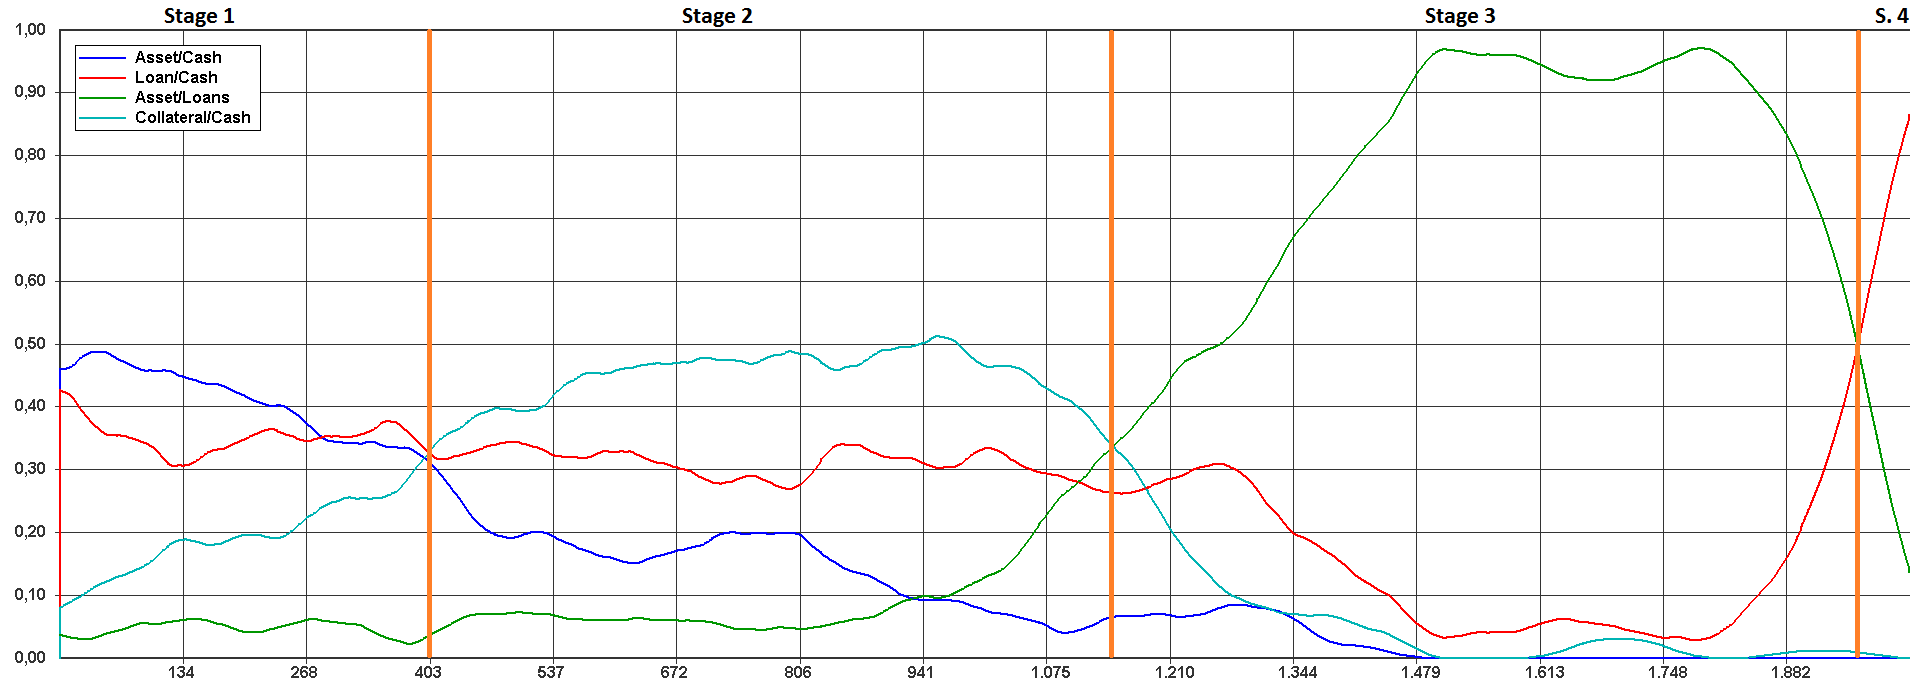
\includegraphics[width=1.0\textwidth, angle=0]{fc/FULLYCONNECTED_100_WITHCOLLATERALMARKET_MARKET_STAGES.png}
  	\caption{Market-activity stages of Fully-Connected topology with Collateral/Cash market}
	\label{fig:markets_FULLYCONNECTED_100_WITHCOLLATERALMARKET_MARKET_STAGES}
\end{figure}

\paragraph{Stage 1}
In this stage the pessimists become visible rapidly as they sell their assets and increase their cash wealth. One can get also a sense of the more optimistic range of agents as they gather assets both free and collateralized. The medianists are not visible yet.

\medskip

The Asset/Cash market dominates but goes down slowly as fewer and fewer pessimists trade assets against cash compared to the very beginning. 
The Bond/Cash market fluctuates around the same point as loans are traded more or less equally the same.
The Collateral/Cash market begins quite low and raises as more and more collateralized assets are created by pessimists and need to be sold again using the new market.
The Asset/Bond market is hardly active as there is no strong need for its features yet.

\begin{figure}[H]
	\centering
  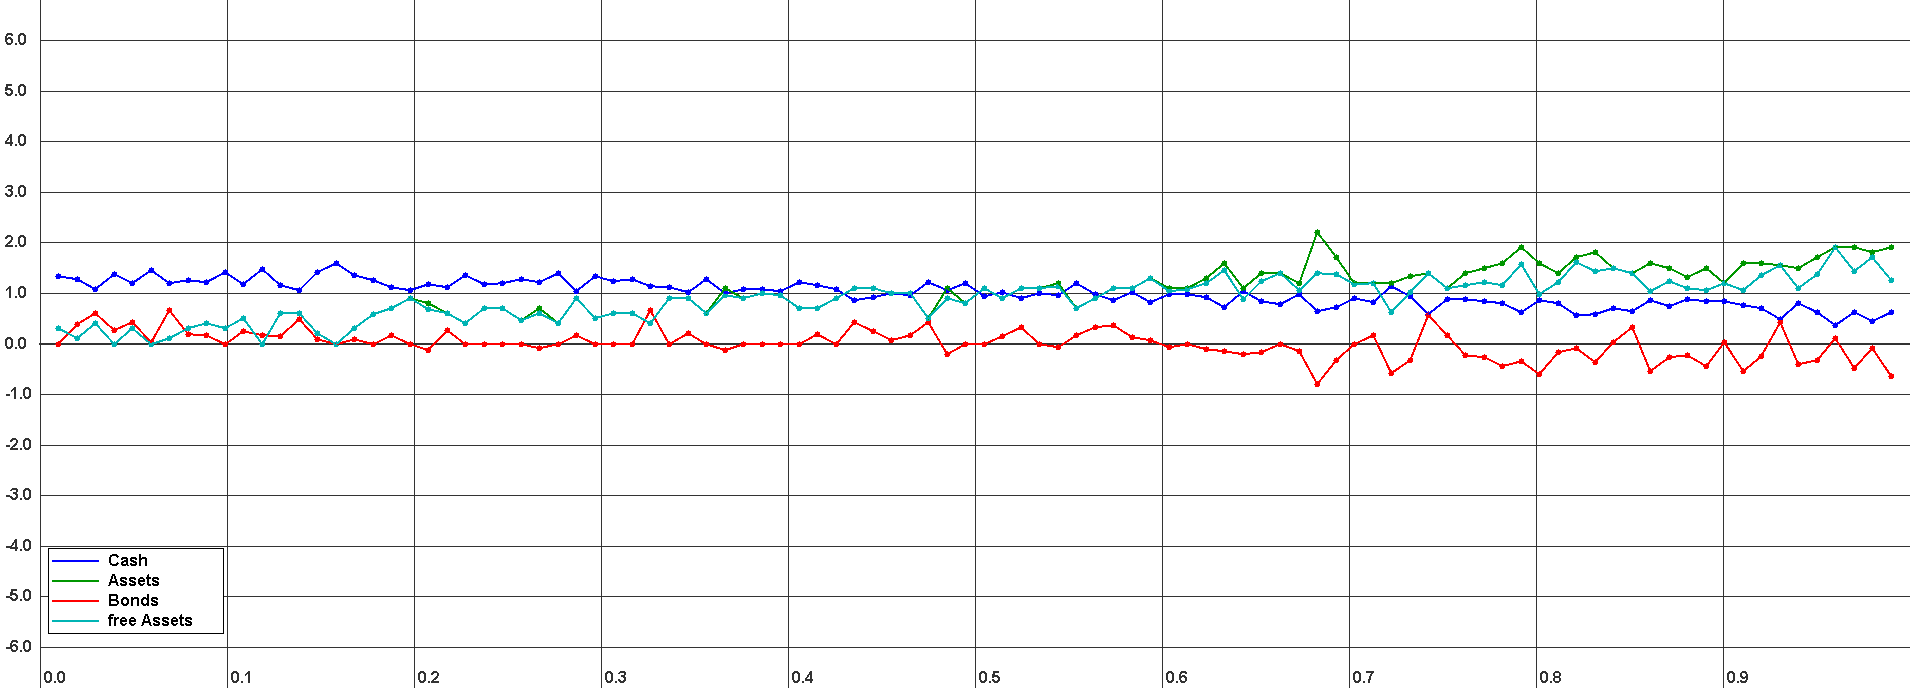
\includegraphics[width=1.0\textwidth, angle=0]{fc/FULLYCONNECTED_100_WITHCOLLATERALMARKET_WEALTH_STAGE_1.png}
  	\caption{Wealth-Distribution of Fully-Connected topology with Collateral/Cash market during Stage 1}
	\label{fig:markets_FULLYCONNECTED_100_WITHCOLLATERALMARKET_WEALTH_STAGE_1}
\end{figure}

\paragraph{Stage 2}
The collateralized assets are traded from the pessimists towards the optimists and the optimists crystallize themselves even more but no medianists are visible yet.

\medskip

The Asset/Cash market continues to go down as the cash holdings of the pessimists begin to decline. The Bond/Cash market fluctuates around the same point as before. Now the Collateral/Cash market becomes very active as more and more collateralized assets need to be traded towards the optimists.
At the beginning of this stage the Asset/Bond market is hardly active but raises fast towards the end of it as the optimists are then out of cash and need to distribute the collateralized assets between each other and the yet to come medianists.

\begin{figure}[H]
	\centering
  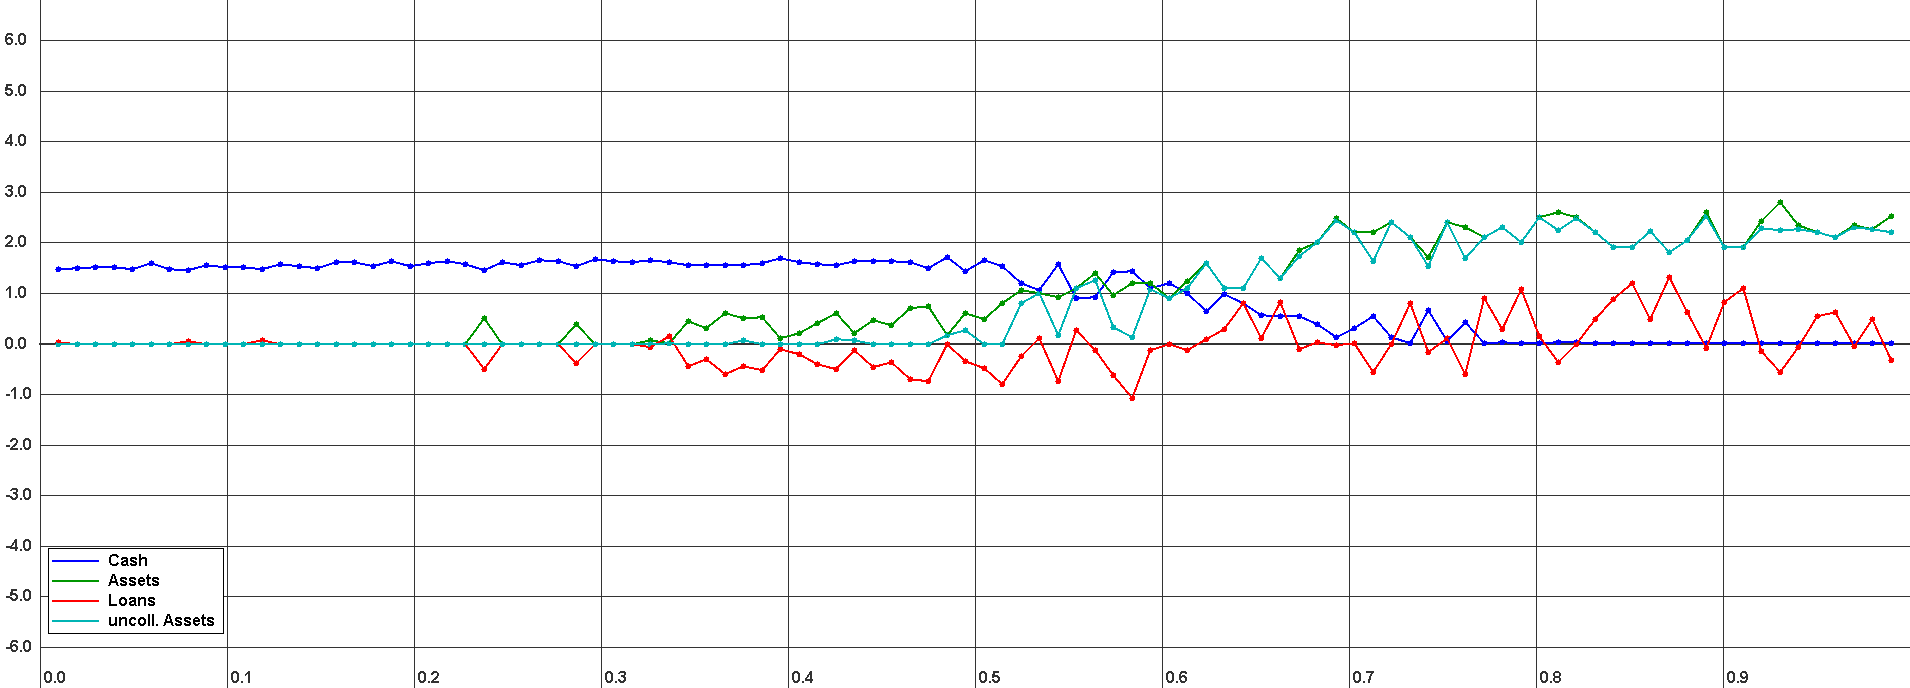
\includegraphics[width=1.0\textwidth, angle=0]{fc/FULLYCONNECTED_100_WITHCOLLATERALMARKET_WEALTH_STAGE_2.png}
  	\caption{Wealth-Distribution of Fully-Connected topology with Collateral/Cash market during Stage 2}
	\label{fig:markets_FULLYCONNECTED_100_WITHCOLLATERALMARKET_WEALTH_STAGE_2}
\end{figure}

\paragraph{Stage 3}
The pessimists have gone inactive as they hold no more wealth they can trade. The i1-point is emerging and the medianists and pure optimists begin to show up.

\medskip

Because the pessimists are inactive now and hold no more assets the Asset/Cash and Collateral/Cash markets go down and decline completely. The Bond/Cash market goes down but does not decline as bonds are still traded because of the emerging of medianists. The medianists and pure optimists which are emerging have no other possibility than to trade on the Asset/Bond market to further distribute their collateralized assets among each other which is the reason for the raise of the Asset/Bond market above all others and its heavy domination. Despite the heavy domination of the Asset/Bond market still a few bonds are traded against cash in the range of the medianists.

\begin{figure}[H]
	\centering
  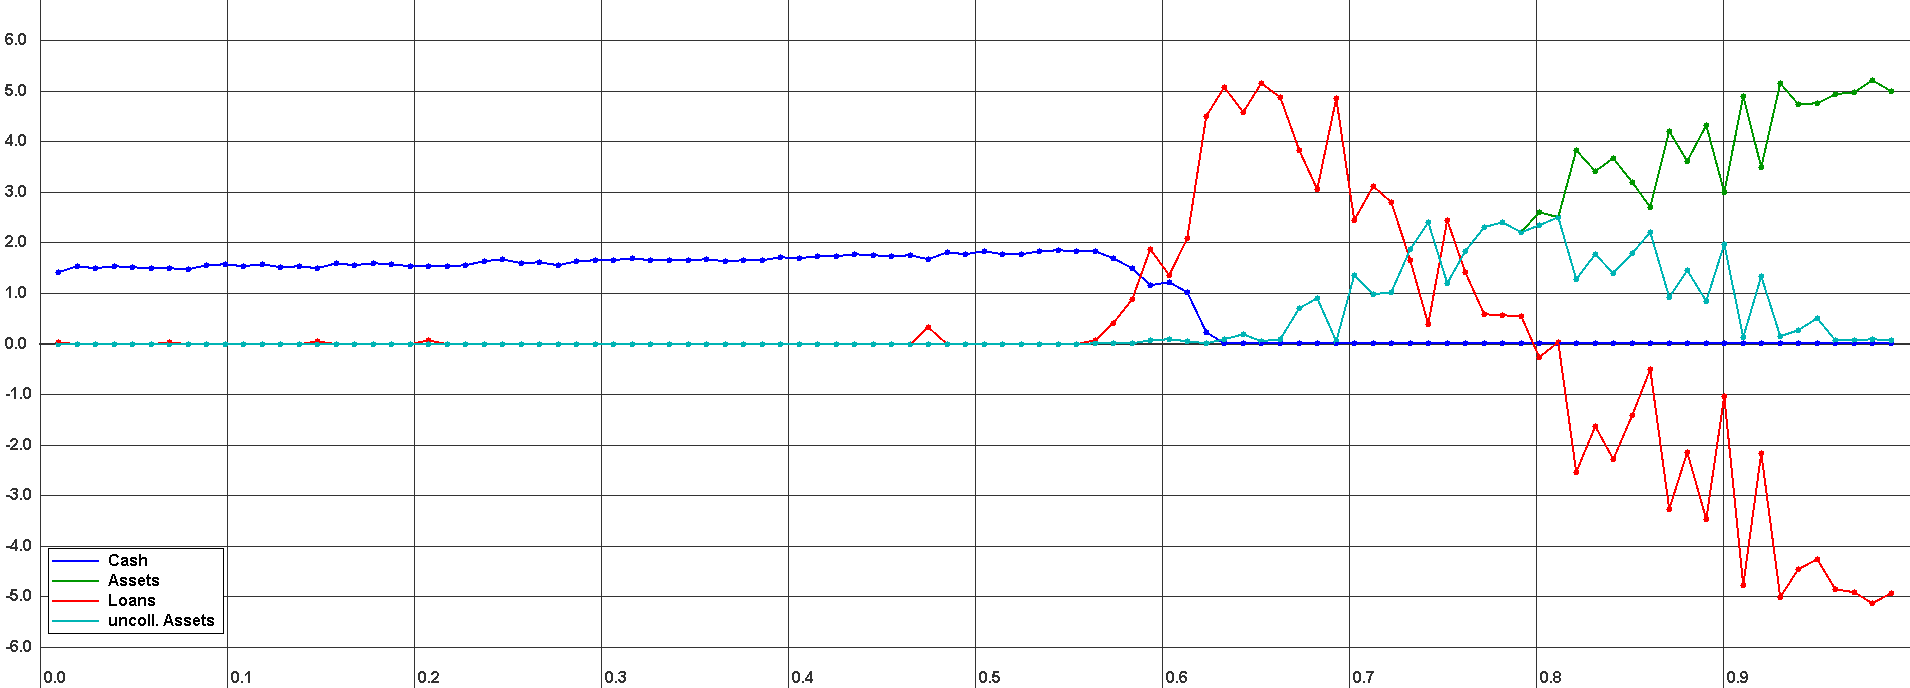
\includegraphics[width=1.0\textwidth, angle=0]{fc/FULLYCONNECTED_100_WITHCOLLATERALMARKET_WEALTH_STAGE_3.png}
  	\caption{Wealth-Distribution of Fully-Connected topology with Collateral/Cash market during Stage 3}
	\label{fig:markets_FULLYCONNECTED_100_WITHCOLLATERALMARKET_WEALTH_STAGE_3}
\end{figure}

\paragraph{Stage 4}
Finally the i2-point has emerged and both i1 and i2 are finalizing. The only active agents remaining are around these two points where the pure optimists trade with the medianists to finalize i2 and the medianists with the next closest pessimists to finalize i1 where the very last transactions occur around i1.

\medskip

The Asset/Bond market goes down until i2 has finalized as the collateralized asset allocation has nearly reached its equilibrium. The Bond/Cash market goes up as agents around i1 are still refining the point as the equilibrium of the medianists is not reached yet. Thus bonds are traded against cash as i1 is the connecting point between pessimists with cash and medianists with bonds which enables the Bond/Cash market to trade again.

\begin{figure}[H]
	\centering
  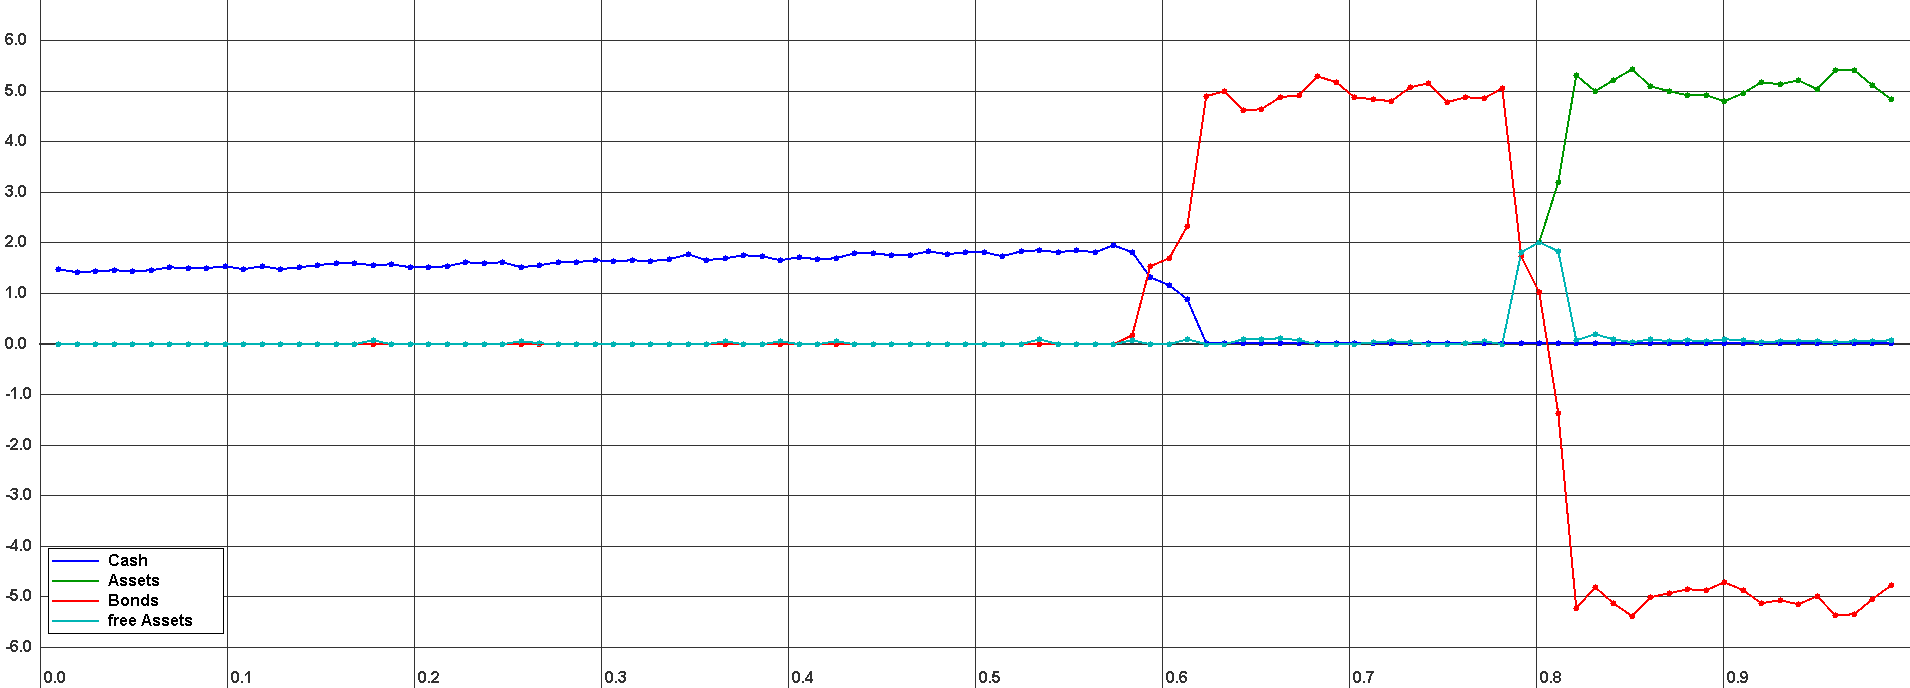
\includegraphics[width=1.0\textwidth, angle=0]{fc/FULLYCONNECTED_100_WITHCOLLATERALMARKET_WEALTH_STAGE_4.png}
  	\caption{Wealth-Distribution of Fully-Connected topology with Collateral/Cash market during Stage 4}
	\label{fig:markets_FULLYCONNECTED_100_WITHCOLLATERALMARKET_WEALTH_STAGE_4}
\end{figure}

\subsection{Deferred new market enabling}
Using the thesis-software it is possible to start a simulation-run on Ascending-Connected topology without the Collateral/Cash market and enabling it after 1,000 successive failed matching-rounds which gives interesting hints about how the spikes of collateralized assets in the pessimists-range are resolved and distributed over the already existing pure optimists.

\medskip

Of course there are the same 3 stages to be found as described already in section \ref{sub:dynamics_singlerun} whereas the deferred enabling of the Collateral/Cash market adds 2 new stages.

\begin{figure}[H]
	\centering
  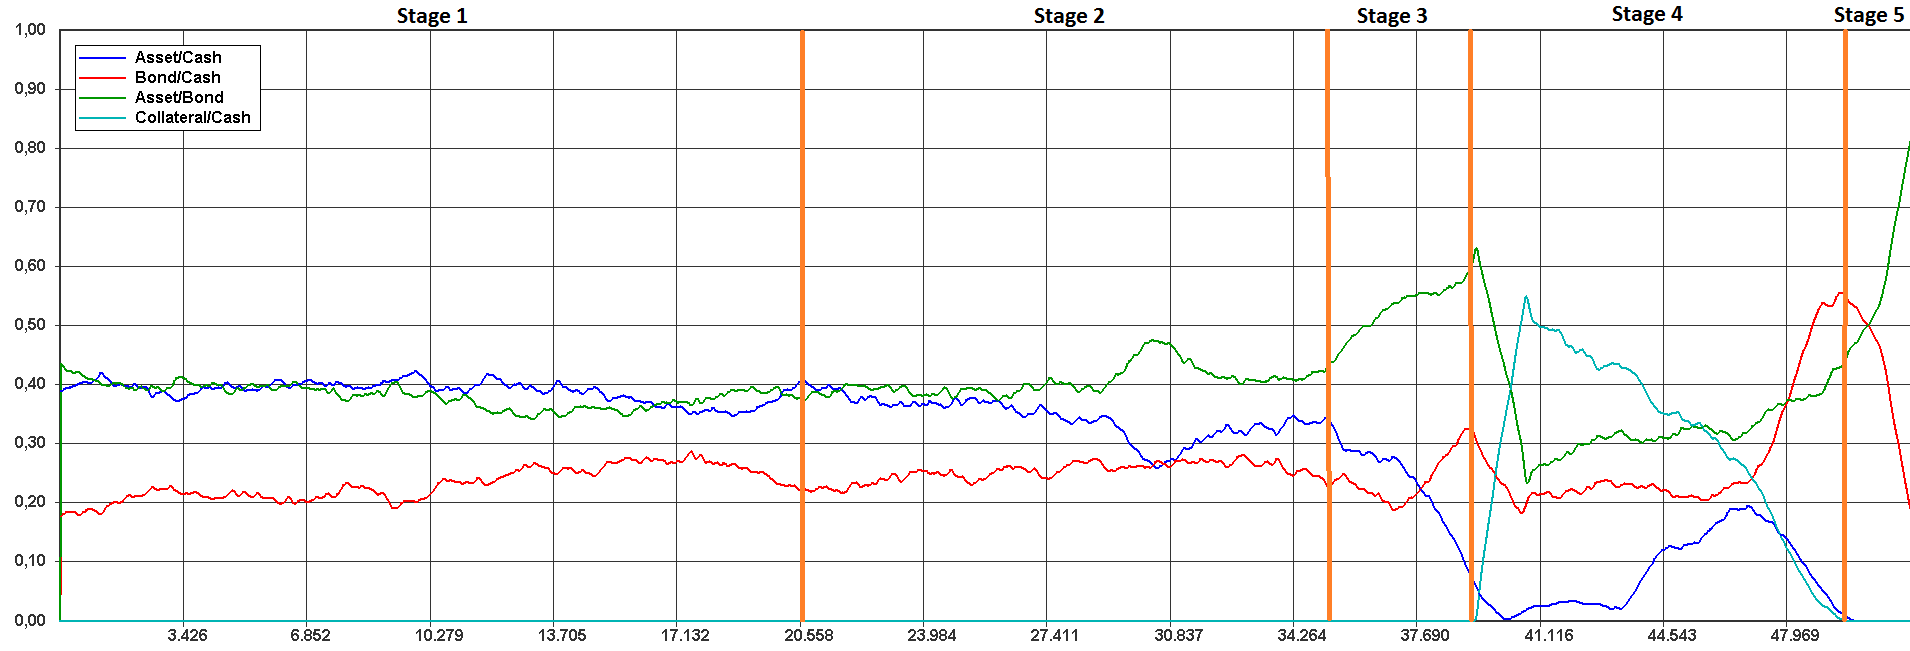
\includegraphics[width=1.0\textwidth, angle=0]{ac/ASCENDINGCONNECTED_100_DEFERREDCOLLATERALMARKET_MARKET_STAGES.png}
  	\caption{Market-activity stages of Ascending-Connected topology with deferred activated Collateral/Cash market}
	\label{fig:markets_ASCENDINGCONNECTED_100_DEFERREDCOLLATERALMARKET_MARKET_STAGES}
\end{figure}

\paragraph{Stage 4}
The collateralized assets are traded against cash and sum up at the i1-point where the first agent has no more cash. 

\begin{figure}[H]
	\centering
  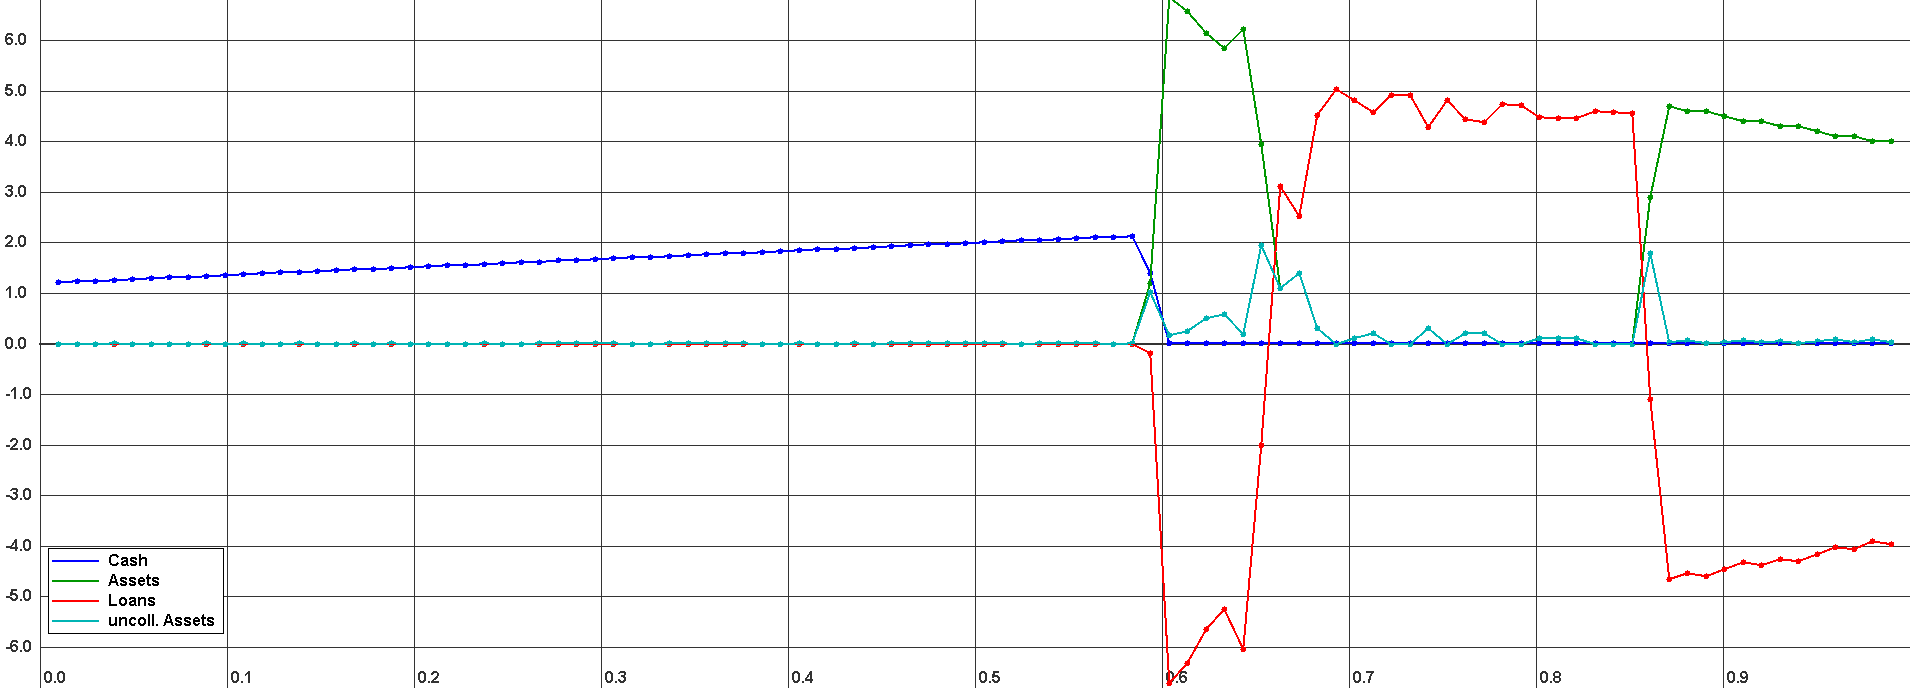
\includegraphics[width=1.0\textwidth, angle=0]{ac/ASCENDINGCONNECTED_100_DEFERREDCOLLATERALMARKET_WEALTH_STAGE_4.png}
  	\caption{Wealth-Distribution of Ascending-Connected topology with deferred activated Collateral/Cash market during Stage 4}
	\label{fig:markets_ASCENDINGCONNECTED_100_DEFERREDCOLLATERALMARKET_WEALTH_STAGE_4}
\end{figure}

\paragraph{Stage 5}
Now the Asset/Bond market becomes 100\% dominant again and the collateralized assets are traded through the medianists towards the pure optimists as they have no more cash and can only trade anymore on this remaining active market.

\begin{figure}[H]
	\centering
  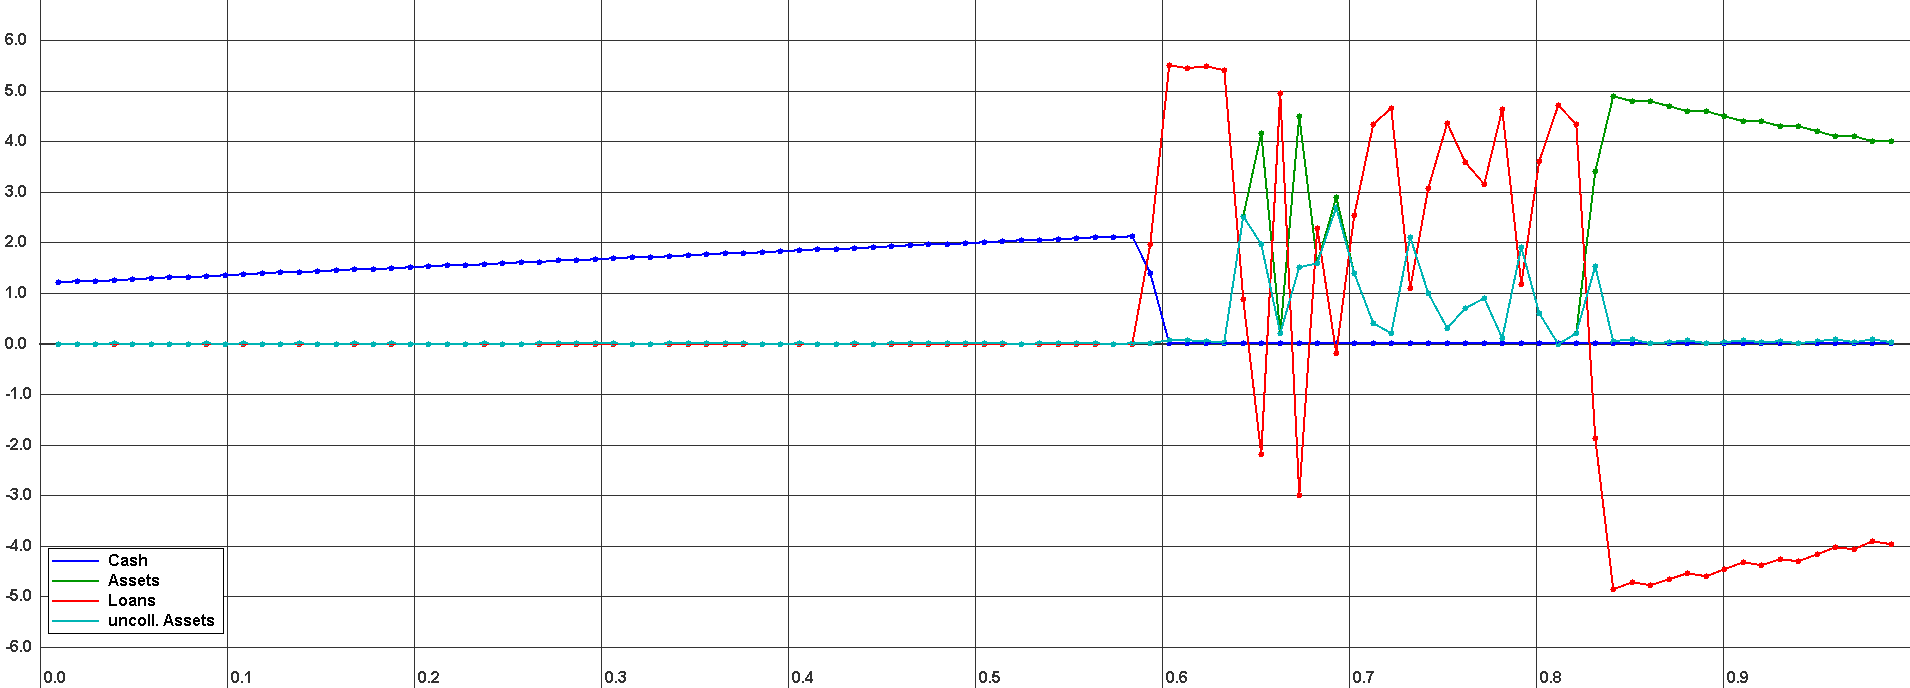
\includegraphics[width=1.0\textwidth, angle=0]{ac/ASCENDINGCONNECTED_100_DEFERREDCOLLATERALMARKET_WEALTH_STAGE_5.png}
  	\caption{Wealth-Distribution of Ascending-Connected topology with deferred activated Collateral/Cash market during Stage 5}	\label{fig:markets_ASCENDINGCONNECTED_100_DEFERREDCOLLATERALMARKET_WEALTH_STAGE_5}
\end{figure}

\subsection{Ascending-Connected with new Market}

4 stages were identified where only 3 of them can be seen in the Market-Dynamics diagram as stage 3 and 4 have indifferent market-activities.

\begin{figure}[H]
	\centering
  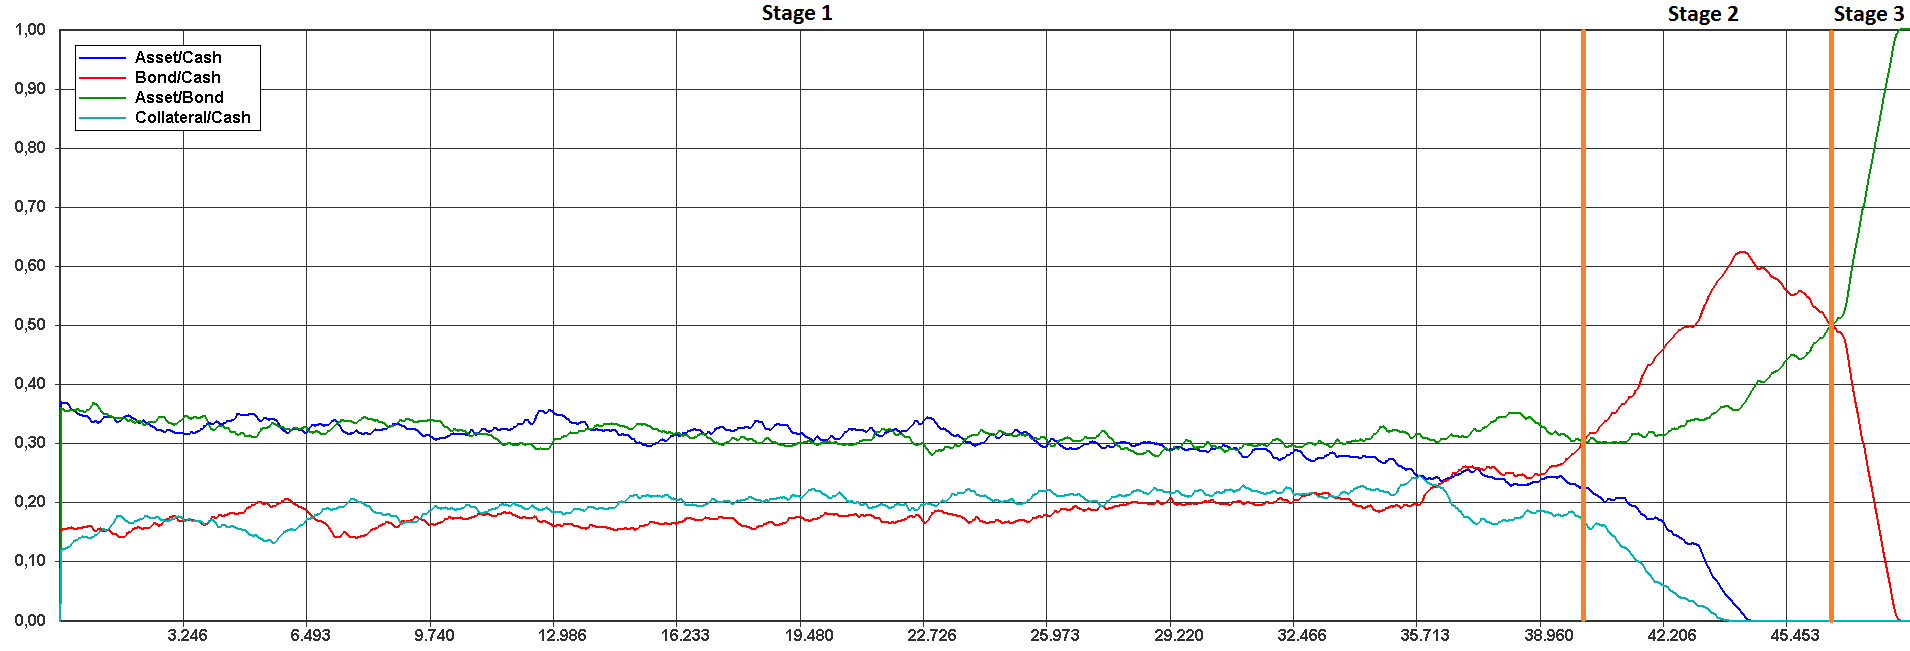
\includegraphics[width=1.0\textwidth, angle=0]{ac/ASCENDINGCONNECTED_100_WITHCOLLATERALMARKET_MARKET_STAGES.png}
  	\caption{Market-activity stages of Ascending-Connected topology with Collateral/Cash market}
	\label{fig:markets_ASCENDINGCONNECTED_100_WITHCOLLATERALMARKET_MARKET_STAGES}
\end{figure}

\paragraph{Stage 1}
Pessimists and optimists begin to emerge where the pessimists are gathering cash and collateralized assets and the optimists are gathering free assets against cash and a few collateralized assets. There are no medianists visible yet.

\medskip

The Asset/Cash and Bond/Cash markets start around 40\% slightly decreasing because the pessimists are slowly going low on assets. The Collateral/Cash market starts around 10\% with increasing tendency because the amount of collateralized assets which move towards the optimists increases. The Asset/Bond market is hardly active as its features are not yet very necessary.
		
\begin{figure}[H]
	\centering
  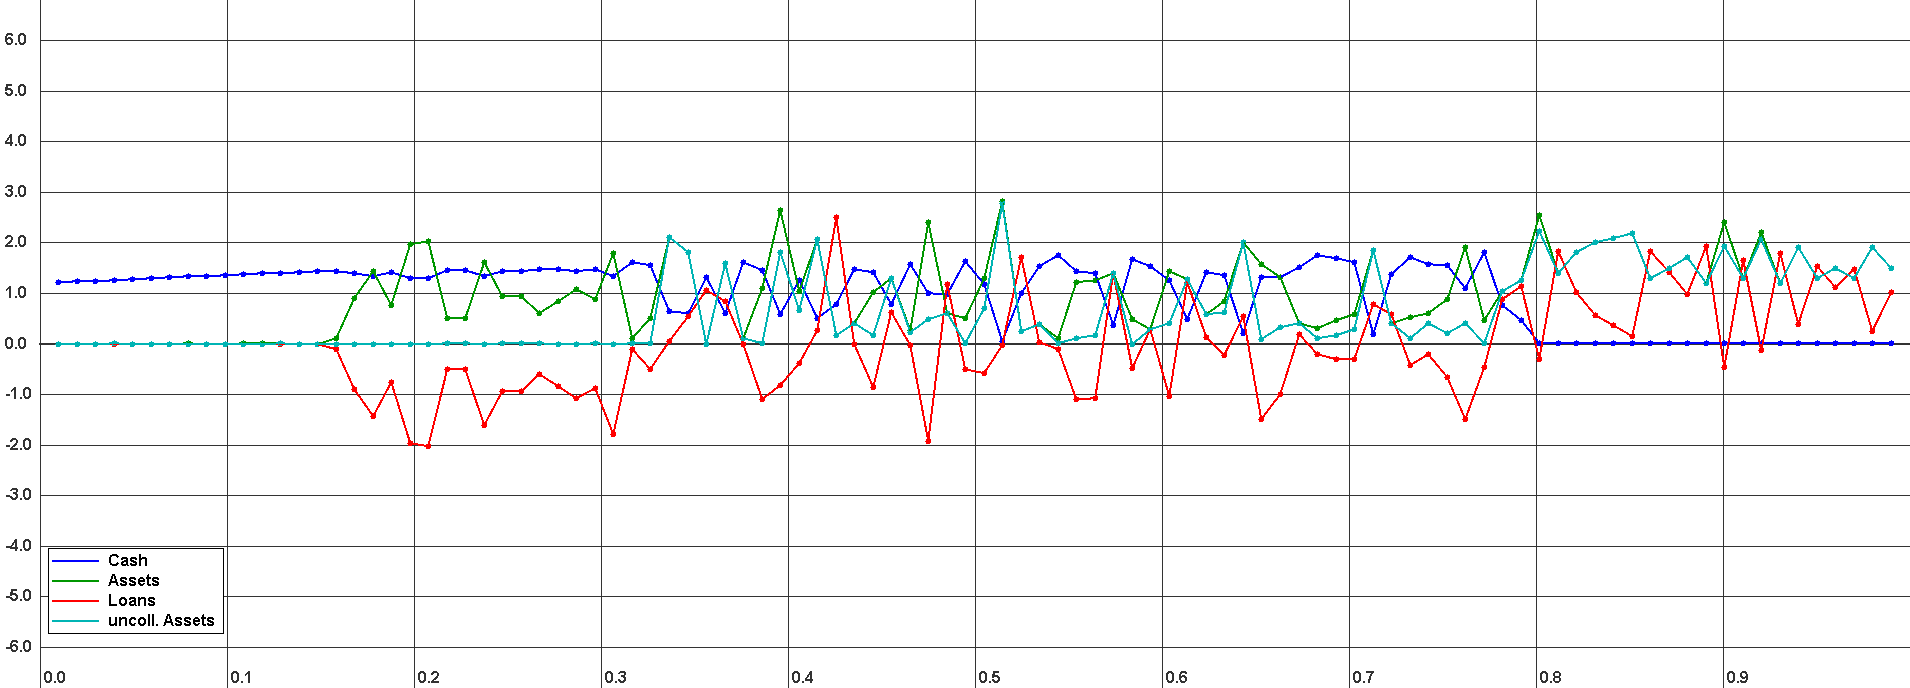
\includegraphics[width=1.0\textwidth, angle=0]{ac/ASCENDINGCONNECTED_100_WITHCOLLATERALMARKET_WEALTH_STAGE_1.png}
  	\caption{Wealth-Distribution of Ascending-Connected topology with Collateral/Cash market during Stage 1}
	\label{fig:wealth_ASCENDINGCONNECTED_100_WITHCOLLATERALMARKET_WEALTH_STAGE_1}
\end{figure}

\paragraph{Stage 2}
In the pessimist-range large amount of collateralized assets have gathered which are traded now towards the optimists as the pessimists try to get maximally short on any assets and maximally plus on cash. Those collateralized assets are traded towards the i1-point - that is the first agent who holds no more cash - which can be seen by a spike in the wealth-distribution of figure \ref{fig:wealth_ASCENDINGCONNECTED_100_WITHCOLLATERALMARKET_WEALTH_STAGE_2} around 0.65.
There are no medianists visible yet.

\medskip

The Collateral/Cash market raises above the Asset/Cash and Bond/Cash markets and either fluctuates or stays quite constant. In figure \ref{fig:markets_ASCENDINGCONNECTED_100_WITHCOLLATERALMARKET_MARKET_STAGES} the fluctuating variant is shown. If the market fluctuates the Asset/Cash and Bond/Cash fluctuate inverse in that if Collateral/Cash market raises they go down and vice versa. If the Collateral/Cash market stays quite constant in this stage it raises above 90\% and Asset/Cash and Bond/Cash markets decline to 0\%. Why the Collateral/Cash market either fluctuates or stays constant is not clear but is most probably dependent on the allocation of collateralized assets in the pessimists-range. The Asset/Bond market becomes a bit more active as more collateralized assets are traded.

\begin{figure}[H]
	\centering
  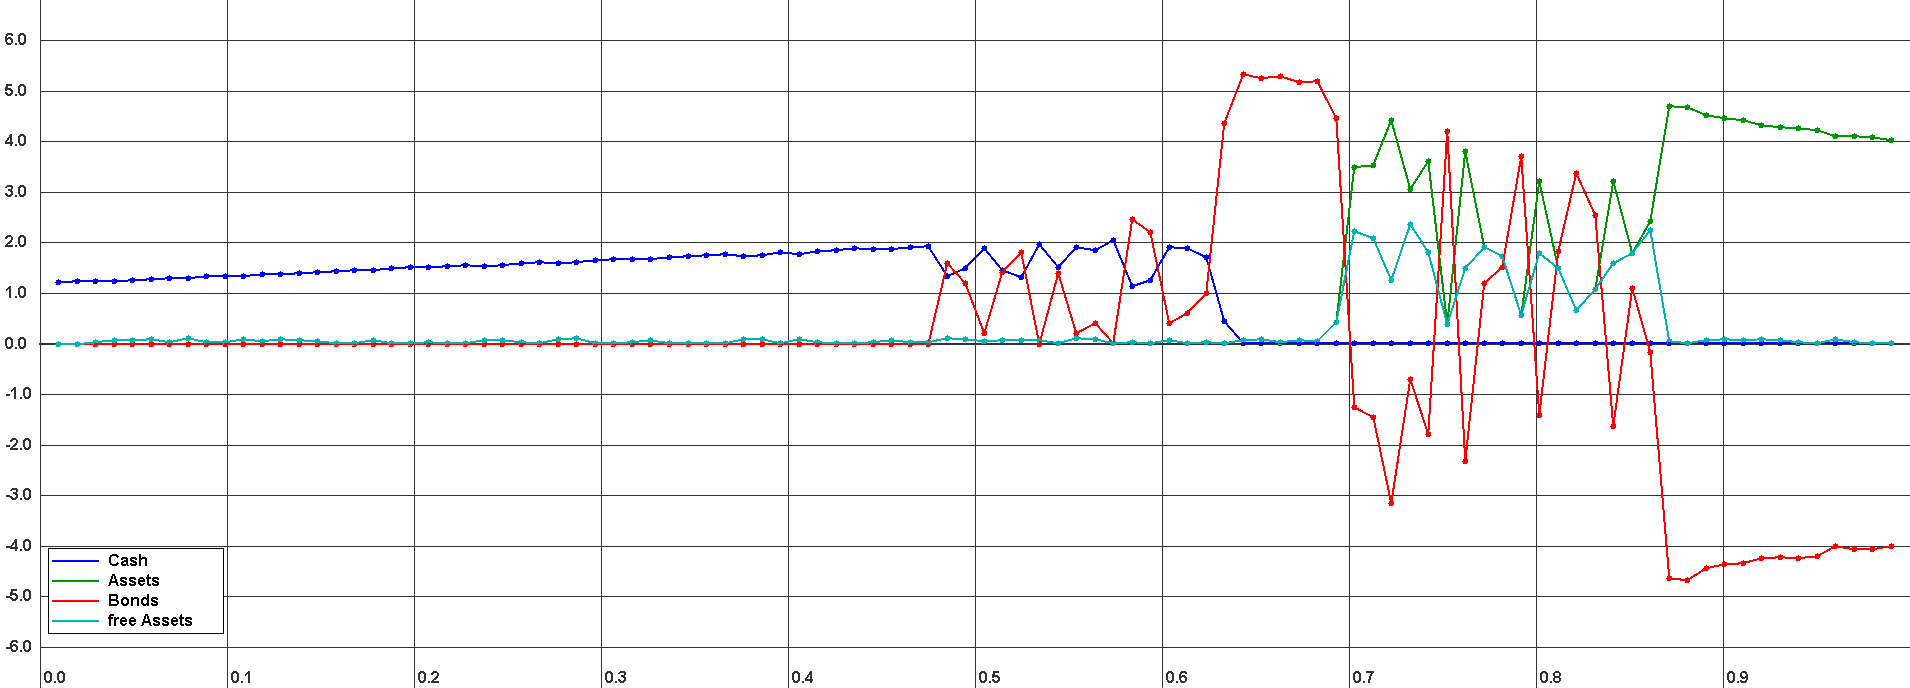
\includegraphics[width=1.0\textwidth, angle=0]{ac/ASCENDINGCONNECTED_100_WITHCOLLATERALMARKET_WEALTH_STAGE_2.png}
  	\caption{Wealth-Distribution of Ascending-Connected topology with Collateral/Cash market during Stage 2}
	\label{fig:wealth_ASCENDINGCONNECTED_100_WITHCOLLATERALMARKET_WEALTH_STAGE_2}
\end{figure}

\paragraph{Stage 3}
Pessimists are now final and won't change any more. The optimists-range is now clearly visible and holds a large amount of collateralized assets from the pessimists which needs now to be traded and distributed to the remaining optimists. Medianists are still not visible yet.

\medskip

Because the pessimists are no more able to trade and the optimists hold no more cash the activity of the Collateral/Cash market drops rapidly and Asset/Bond market raises to 100\% activity as only collateralized-assets are tradeable any more.

\begin{figure}[H]
	\centering
  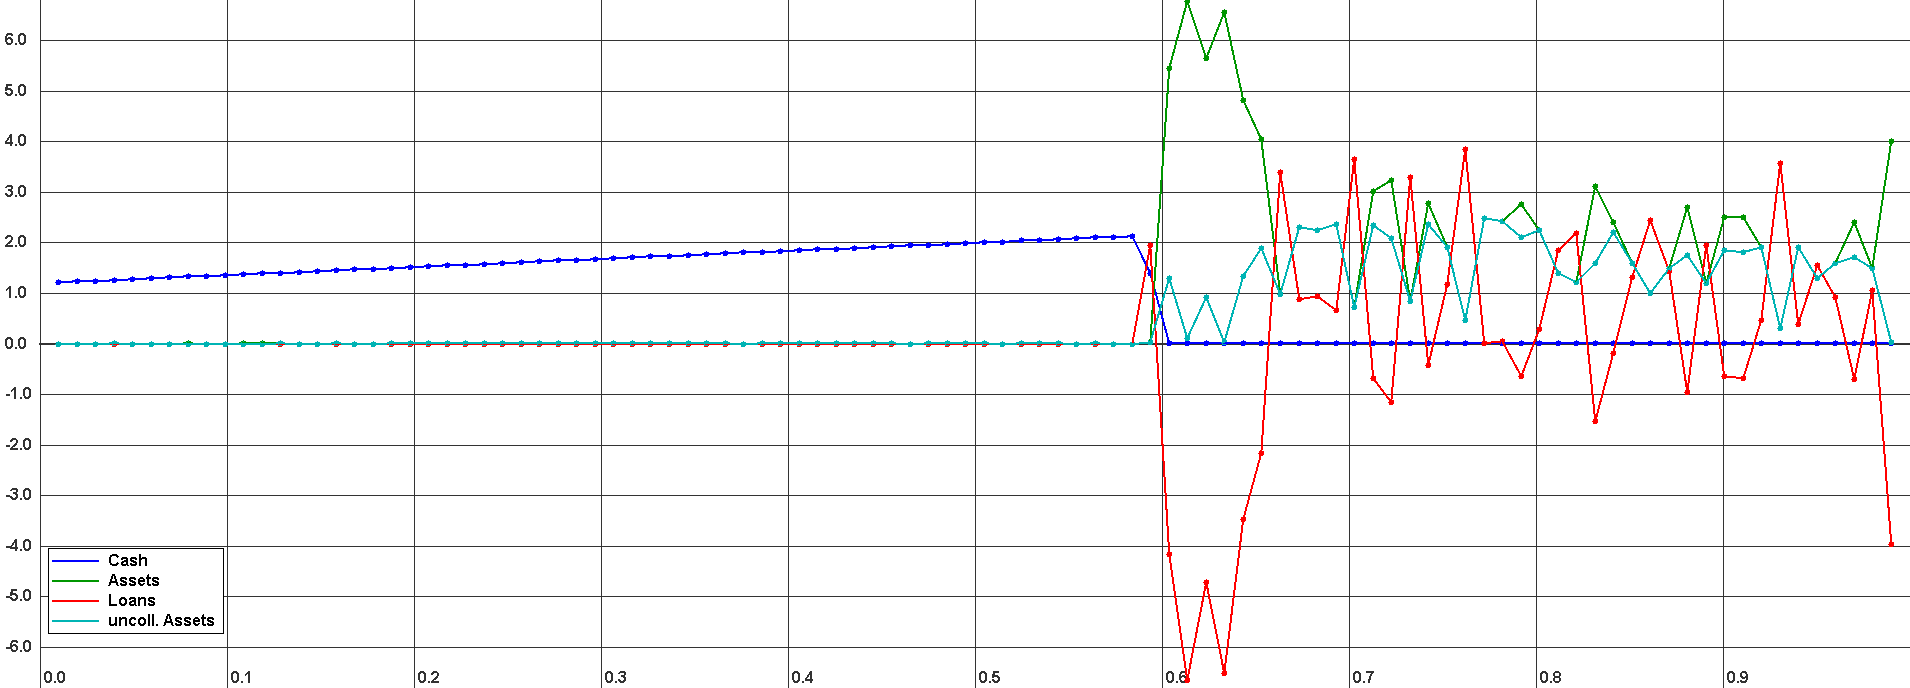
\includegraphics[width=1.0\textwidth, angle=0]{ac/ASCENDINGCONNECTED_100_WITHCOLLATERALMARKET_WEALTH_STAGE_3.png}
  	\caption{Wealth-Distribution of Ascending-Connected topology with Collateral/Cash market during Stage 3}
	\label{fig:wealth_ASCENDINGCONNECTED_100_WITHCOLLATERALMARKET_WEALTH_STAGE_3}
\end{figure}

\paragraph{Stage 4}
Medianists begin to show up and to distinguish themselves from the pure optimists. This is no more visible on the market-dynamics as only Asset/Bonds are traded any more and thus only this market is active any more.

\begin{figure}[H]
	\centering
  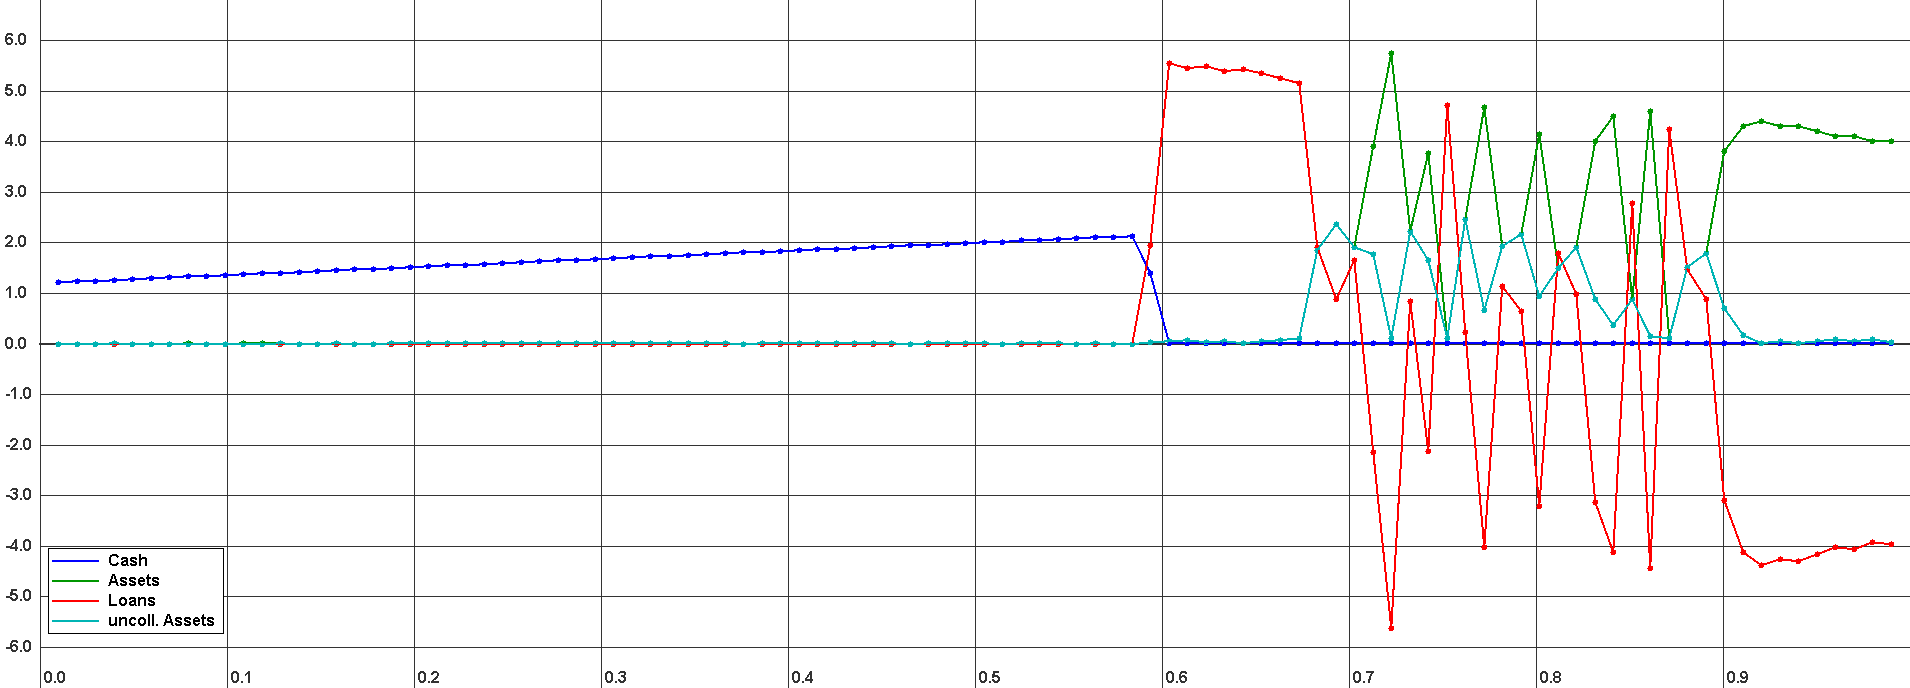
\includegraphics[width=1.0\textwidth, angle=0]{ac/ASCENDINGCONNECTED_100_WITHCOLLATERALMARKET_WEALTH_STAGE_4.png}
  	\caption{Wealth-Distribution of Ascending-Connected topology with Collateral/Cash market during Stage 4}
	\label{fig:wealth_ASCENDINGCONNECTED_100_WITHCOLLATERALMARKET_WEALTH_STAGE_4}
\end{figure}

After these observations made one can answer the questions.

\paragraph{Can the trading stages 1-4 be identified too as given in \cite{Breuer2015}?}
There are 4 stages in the case of both Fully-Connected and Ascending-Connected topology with the new market which are not the ones given in \cite{Breuer2015} but show up by pure chance and depend also a bit on the point-of-view on how to separate the stages from each other. 

\paragraph{How does trading progress with this new market? Is it the same as without the new market?}
The progression of the trading is obviously very different with the new market as compared to the market-activities without as the usage of the new market changes the dynamics completely.

\paragraph{How does the new market resolve the miss-allocation (with and without deferred activation)?}
It becomes active during the formation of the pessimists agents as they gather collateralized assets wealth which must be traded towards the optimists. The collateralized assets are traded from neighbour to neighbour until they reach the optimists-region.

\paragraph{When and how much is each market active?}
This can be seen clearly in the market-activity diagrams.

\paragraph{How do the market-activities change when a new market is introduced?}
They have less share on the overall activity and thus the new market is quite a heavy competitor in the overall share. The Asset/Bond market though is still the market on which the final trades occur.

\section{Conclusions on new Market}
The equilibrium of the Ascending-Connected topology with the new market is different than the Fully-Connected one which reaches the theoretical equilibrium. Thus the hypothesis is still wrong because it predicted the Ascending-Connected topology to reach the theoretical equilibrium. This thesis can only speculate on the reason for this it is most probably rooted in the fundamental different trading dynamics of Ascending-Connected topology compared to Fully-Connected as can be seen in the market-dynamics. This thesis leaves the question of market-dynamics open for further research.

\end{document}
